%
%    18afmc template paper adapted from 14afmc template.
%
%    Format: LaTeX2e.
%
\ifcase0 %case 0 is for my drafts (15pp should be OK)
\documentclass[a5paper,12pt]{article}
\usepackage[a5paper,tmargin=15mm,bmargin=15mm]{geometry}
\addtolength{\textwidth}{2.7em}% width is about right
\let\affiliation\date
\or %case 1 is for the real thing
\documentclass[twocolumn]{afmc_art}
\fi
\usepackage[author=AJR]{pdfcomment}
\AtBeginDocument{\listofpdfcomments}
\usepackage{amsmath,defns}
\usepackage{url,graphicx,microtype}
\usepackage{hyperref} 
\hypersetup{pdftex,
            backref=true,
            hyperindex=true,
            colorlinks=true,
            citecolor=blue,
            bookmarks=true,
            breaklinks=true}
%
%%%  Fill in following information.
%
%%%%%%%%%%%%%%%%%%%%%%%%%%%%%%%%%%%%%%%%%%%%%%%%%%%%%%%%%%%%%%%%%%%%%%%%%%%%
%
%    Contact Author: Meng Cao
%            E-mail: meng.cao@adelaide.edu.au
%             Phone: +61 8 8313 1606
%               Fax:+61 8 8313 3696
%
%%%%%%%%%%%%%%%%%%%%%%%%%%%%%%%%%%%%%%%%%%%%%%%%%%%%%%%%%%%%%%%%%%%%%%%%%%%%
%
%%%  Put your definitions (if any) here
\allowdisplaybreaks
\newcommand{\zs}{\zeta}
\newcommand{\uu}{{\bar u}}
\newcommand{\vv}{{\bar v}}
\newcommand{\bq}{{\bar q}}
\newcommand{\qq}{{\bar{\vec q}}}
\newcommand{\ee}{\textsc{e}}
\newcommand{\rnu}{R_\nu}
\newcommand{\ros}{{\dot\varepsilon}}
\renewcommand{\vec}[1]{\text{\boldmath$#1$}}
%
%%%  Title goes here - do not force a line-break unless ABSOLUTELY necessary
%

\title{Modelling 3D turbulent floods based upon the Smagorinski large eddy closure}

\author{Meng Cao$^1$ and A.~J. Roberts$^1$}
\affiliation{$^1$School of Mathematical Sciences\\
                University of Adelaide, South Australia 5005, Australia\\[5pt]
            }
%\date{31 May 2012}

\begin{document}
    
\maketitle

\section{Abstract}
Rivers, floods and tsunamis are often very turbulent.
Conventional models of such environmental fluids are typically based on depth averaged inviscid irrotational flow equations.
We explore the implications of changing the theoretical base to the turbulent Smagorinski large eddy closure.
The aim is to more appropriately model the fluid dynamics of such complex environmental fluids by using such a turbulent closure.
Large changes in fluid depth are allowed.
Computer algebra constructs the slow manifold of the flow in terms of the fluid depth and the mean turbulent lateral velocities.
The major challenge is to deal with the nonlinear stress tensor in the Smagorinski closure.
The model integrates the effects of inertia, self-advection, bed drag, gravitational forcing and turbulent dissipation with minimal assumptions.
Although the resultant model is close to established models, the real outcome is creating a sound basis for the modelling so others, in their modelling of more complex situations, can systematically include more complex physical processes.

\textbf{Keywords}\quad turbulent flood, tsunami, Smagorinski closure, channel flows

\section{Introduction}

Environmental turbulent fluids have large wave length compared with the fluid depth.
%Large eddy viscosity model is always used to account for the turbulence.
Bousmar~\cite{Bousmar2002}, Liu et al.~\cite{Liu2009}, Demuren~\cite{Demuren1993} and others experimentally and numerically explored compound channel flows as being typical of such environmental turbulent fluid.
Conventional mathematical models of such flows are carried out by depth averaging the flow equations. 
Bousmar~\cite{Bousmar2002} proposed an exchange discharge model~(\textsc{edm}) by depth averaging the Navier--Stokes equations.
The~\textsc{edm} solves the momentum transfers experimentally and numerically through the turbulent exchange and geometrical transfer between channel subsections, the channel and the shallow regions.
The~\textsc{edm} predicts the discharge and water profile computation successfully and supports our simulations of flows along straight channels. 
Liu et al.~\cite{Liu2009} simulated shallow water flows in curved and meandering channels by a depth averaged lattice Boltzmann model by using the large eddy simulation model to account for turbulence.
Our simulations of flows over meandering channels are compared with those of Liu et al.~\cite{Liu2009}. 

However, Roberts~\cite{Roberts1996} discussed evidence that the depth averaging in such models is quantitatively unsound.
Here we resolve some of the turbulent dynamics using the Smagorinski model.
But instead of depth averaging flow equations, we obtain low order models based upon centre manifold theory. 
The theory assures that there exists an emergent low dimensional, slow manifold for the evolution governed by the continuity equation~\eqref{eq:cont}, momentum equation~\eqref{eq:mom} and nonlinear shear tensor in the Smagorinski closure~\eqref{eq:stress}.
The resulting model is then used to simulate flows over straight and meandering compound channels and to compare with published data~\cite[e.g.]{Bousmar2002, Liu2009}.


\section{Detailed equations of the turbulent model}

Let's consider three dimensional incompressible and irrotational turbulent fluid flowing down a slightly sloping ground. 
Define Cartesian coordinates with the lateral directions $x_1=x$ and $x_2=y$ and the normal direction $x_3=z$. 
Let the turbulent fluid have thickness~$h(x,y,t)$ over the ground located at $z=b(x,y)$ with a mean slope~$\theta$ in the $x=x_1$ direction, denote the turbulent mean velocity field by $\vec q(x,y,z,t)=(u,v,w)=(u_1,u_2,u_3)$, and the turbulent mean pressure field by~$p(x,y,z,t)$.
After non-dimensionalising the variables with respect to a typical fluid thickness~$H$, the velocity scale~$\sqrt{gH}$, and the  fluid density, the non-dimensional governing partial differential equations for the incompressible, irrotational, three dimensional, turbulent mean fluid fields are the continuity equation
\begin{equation}
    \divv\vec q=\D xu+\D yv+\D zw=0\,,\label{eq:cont}
\end{equation}
and the momentum equation
\begin{equation}
    \D t{\vec q} +\vec q\cdot\grad\vec q
    =-\grad p +\divv\tau +\vec{g}\,,\label{eq:mom}
\end{equation}
where~$\tau$ is the turbulent mean stress tensor, and $\vec g=(g_1,0,g_3)$ is the forcing from gravity ($|\vec g|=1$ by the non-dimensionalisation).
In the Smagorinski model the effects of turbulence are modelled by via an eddy viscosity~$\nu$, which is related to the mean shear stress through the mean stress-strain equation of
\begin{equation}
\tau_{ij}=2\nu\ros_{ij}\,,\label{eq:tau}
\end{equation}
with the indexes $i,j=1,2,3$ indicating in the $x$, $y$ and~$z$ directions.
Define the turbulent mean strain-rate tensor~\cite[e.g.]{Roberts2008,Georgiev2008}
\begin{equation}
	\ros_{ij} =\frac12\left( \D{x_j}{u_i} +\D{x_i}{u_j}\right) \,,\label{eq:strainrate}
\end{equation}
and then the non-dimensional turbulent mean stress tensor for the turbulent fluid is
\begin{equation}
\sigma_{ij}=-p\delta_{ij}+2\nu\ros_{ij}\,.\label{eq:sigma}
\end{equation}
When the eddy viscosity~$\nu$ is constant, equation~\eqref{eq:sigma} models a Newtonian fluid.
In the Smagorinski model~\cite[e.g.]{Ozgokmen2007a}, the eddy viscosity~$\nu$ varies linearly with the magnitude~$\ros$ of the second invariant of the strain-rate tensor,
\begin{equation}
  \nu=c_th^2\ros\quad\text{where}\quad |\ros|^2=\sum_{i,j}\ros_{ij}^2\,.\label{eq:nu}
\end{equation}
Roberts et al.~\cite{Roberts2008} recommended the proportionality constant $c_t\approx0.02$ for turbulent environmental flows through comparison with established channel flow experiments~\cite[e.g.]{Nezu2005}.
Thus, equations~\eqref{eq:tau}--\eqref{eq:nu} give the turbulent mean stress tensor
\begin{equation}
\tau_{ij}=2\nu(\ros)\ros_{ij}=c_th^2\ros\left( \D{x_j}{u_i} +\D{x_i}{u_j}\right) \,.\label{eq:stress}
\end{equation}
We formulate boundary conditions on the ground $z=b(x,y)$ and free surface $z=\eta(x,y,t)=h(x,y,t)+b(x,y)$ in terms of the turbulent mean velocity field~$\vec q(x,y,z,t)$ and the fluid depth~$h(x,y,t)$. 
On the ground, no fluid penetrating the ground requires $\vec q\cdot\vec n=0$\,:
\begin{equation}
w=ub_x+vb_y \quad\text{on } z=b\,,
\label{eq:nopen}
\end{equation}
where the unit normal vector to the ground is
\begin{equation}
\vec n=(-b_x,-b_y,1)/\sqrt{1+b_x^2+b_y^2}.
\label{eq:vecn}
\end{equation} 
We posit a slip law on the ground to account for a negligibly thin turbulent boundary layer:
\begin{equation}
\vec q_{\text{tan}}=c_uh\frac{\partial\vec q_{\text{tan}}}{\partial n} \quad\text{on } z=b\,,
\label{bc:slip}
\end{equation} 
where $\vec q_{\text{tan}}$ represents the velocity tangential to the ground. 
Roberts et al.~\cite{Roberts2008} found the constant $c_u\approx1.85$ matched open channel flow observations. 
In a wider range of applications, the coefficient~$c_u$ would change for different ground roughness. 
Unit vectors tangential to the ground in the $x$~and~$y$ directions are
\begin{equation*}
\vec t_x=\frac{1}{\sqrt{1+b_x^2}}(1,0,b_x)
\quad\text{and}\quad
\vec t_y=\frac{1}{\sqrt{1+b_y^2}}(0,1,b_y).
\end{equation*}
The boundary condition~\eqref{bc:slip} on the ground \(z=b\) becomes
\begin{align}&
\frac{1}{\sqrt{1+b_x^2}}(u+wb_x)=\frac{c_uh}{\sqrt{1+b_x^2+b_y^2}}\D n{}(u+wb_x)\,,\label{slip:u}\\&
\frac{1}{\sqrt{1+b_y^2}}(v+wb_y)=\frac{c_uh}{\sqrt{1+b_x^2+b_y^2}}\D n{}(v+wb_y)\,.\label{slip:v}
\end{align}
On the free surface (that is, on its turbulent mean position), the kinematic condition is 
\begin{equation}
 \D{t}{\eta}+u\D{x}{\eta}+v\D{y}{\eta}=w \quad\text{on } z=\eta=h+b\,,
\end{equation}
Relative to atmospheric pressure, the pressure on the free surface is zero. 
Thus the turbulent mean stress normal to the free surface is also zero: on $z=\eta$,
\begin{equation}
    -p+\frac{\tau_{33} -2\eta_x\tau_{13} -2\eta_y\tau_{23}
    +\eta_x^2\tau_{11} +2\eta_x\eta_y\tau_{12}+\eta_y^2\tau_{22}}
    {1+\eta_x^2+\eta_y^2}
     =0\,.
    \label{bc:ttz}
\end{equation}
There must be no turbulent mean, tangential stress at the free surface: namely the following for the case of parameter $\gamma=1$\,,
\begin{eqnarray}&&
    (1-\eta_x^2)\tau_{13}+\eta_x(\tau_{33}-\tau_{11})
    -\eta_y(\tau_{12}+\eta_x\tau_{23})
    \nonumber\\&&{}
    = \frac{(1-\gamma)\sqrt2c_t}{(1+c_u)(1+2c_u)} u\sqrt{u^2+v^2}
    \quad\text{on } z=\eta\,,
    \label{bc:ttx}
    \\&&
    (1-\eta_y^2)\tau_{23}+\eta_y(\tau_{33}-\tau_{22})
    -\eta_x(\tau_{12}+\eta_y\tau_{13})
    \nonumber\\&&{}
    = \frac{(1-\gamma)\sqrt2c_t}{(1+c_u)(1+2c_u)} v\sqrt{u^2+v^2}
    \quad\text{on } z=\eta\,.
    \label{bc:tty}
\end{eqnarray}


\section{Reduced model of the fluid dynamics}

This section focusses on interpreting the application of centre manifold theory and the resulting modelling of the turbulent flow.
Instead of depth averaging equations, we apply centre manifold theory to deal with the turbulent dynamics across the fluid layer. 
Roberts, Georgiev and Strunin~\cite{Roberts2008, Georgiev2008} detailed similar approaches by introducing the parameter~$\gamma$ into the free surface tangential stress conditions~\eqref{bc:ttx} and~\eqref{bc:tty} where $\gamma=0$ empowers analytic analysis and approximation, whereas $\gamma=1$ recovers the physical case. 
As described in previous research~\cite{Roberts2008, Georgiev2008}, when parameter \(\gamma=0\) lateral shear modes of turbulent flow become neutral modes of the dynamics, that is, they form a slow subspace along with conservation of fluid.
Centre manifold theory~\cite[e.g.]{Vanderbauwhede88} then assures us that there exists a slow manifold, that we can construct, of the nonlinear dynamics and under changes in the parameters.
Evaluating the resulting slow manifold model at the real case of parameter \(\gamma=1\) then provides a model for the fluid dynamics.
 
Roberts~\cite{Roberts:2008fk}, in a freely available report, detailed the computer algebra that constructed the slow manifold model in 2D flow. 
Modifications for 3D~flow empowers the computer algebra program to derive the evolutions of the water depth~$h(x,y,t)$ and the depth averaged lateral velocities $\uu(x,y,t)$~and~$\vv(x,y,t)$. 
In the centre manifold framework we can choose any reasonable measure of the fluid dynamics in order to parametrise the model: we \emph{choose} the depth averaged lateral velocities and fluid depth. 
We let $\bq(x,y,t)=\sqrt{\uu^2+\vv^2}$ denote the depth averaged speed of the fluid flow.
Omitting the intricate details of the derivation, the evolution of~$h(x,y,t)$, $\uu(x,y,t)$ and~$\vv(x,y,t)$ are described by the fluid conservation equation and by effective lateral momentum equations:
\begin{align}
\D{t}{h}&
\approx-\D{x}{h\bar u}-\D{y}{h\bar v}\,,\label{smag:h}
\\
\D{t}{\bar u}&
\approx-0.00293 \frac{\bar u\bq}{h}
+0.993\left(g_x-g_z\D{x}{h}-g_z\D{x}{b}\right)
\nonumber\\&
-1.030\bar v\D{y}{\bar u}
-1.045\bar u\D{x}{\bar u}
-0.0115\uu\D{y}{\vv}
+0.0136 \vv\D{y}{\uu}
\nonumber\\&
+0.0030 \uu\D{y}{\vv}
+0.0204 \uu\D{x}{\uu}
+0.237h\bq\DD y\uu
+0.0266h\bq\DD x\uu\,,
\pdfcomment{There does not seem to be enough symmetry between the second order terms of the u equation and the v equation.  Needs checking??  Needs something on why this set of terms??  Note: for 'small' terms should probably only use at most a couple of sig. digits in the coefficients.}
\label{smag:u}
\\
\D{t}{\bar v}&
\approx-0.00293 \frac{\bar v\bq}{h}
-0.993g_z\left(\D{y}{h}+\D{y}{b}\right)
-1.042\bar v\D{y}{\bar v}
\nonumber\\&
-1.026\bar u\D{x}{\bar v}
+0.0037\uu\D y\uu
-0.0152\vv\D x\uu
+0.0167 \vv\D y\vv
\nonumber\\&
+0.0097 \uu\D x\vv
-0.0038 \uu\D y\uu
+0.0068 \vv\D x\uu
\nonumber\\&
+0.249h\bq\DD y\vv
+0.0060h\bq\DD x\vv
+0.256h\bq\D x\uu\D y\uu
\,.\label{smag:v}
\end{align}
Equations~\eqref{smag:h}--\eqref{smag:v} are a result of taking into account the relatively slow variations in the lateral directions $x$~and~$y$ via small but non-zero lateral derivatives $\partial_x$~and~$\partial_y$.  
They are a form of slowly varying approximations~\cite[e.g.]{Roberts1996}.
The momentum equations~\eqref{smag:u} and~\eqref{smag:v} incorporate inertial terms~$\qq_t$, self-advection terms~$\qq\D x\qq$,
\pdfcomment{Might need to be more careful here with self advection??}
bed drag terms~$\bq{\qq}/{h}$, gravitational forcing $g_x-g_z{\grad(h+b)}$, and other terms related to the turbulent mixing, where $\qq=(\uu,\vv)$. 
Although equations~\eqref{smag:h}--\eqref{smag:v} are expressed in terms of depth averaged lateral velocities, they are derived not by depth averaging, but instead by systematically accounting for interaction between vertical profiles of the velocity and the stress and bed drag and lateral space variations. 
The form and coefficients in equations~\eqref{smag:h}--\eqref{smag:v} are supported by dynamical systems theory: the detail in the equations reflects that a slow manifold is in principle composed of exact solutions of the full dynamics and hence accounts for all interactions up to a given order of analysis no matter how small the numerical coefficient in the interactions.

In practice one might only implement those terms of equations~\eqref{smag:h}--\eqref{smag:v} which are important in a specific application.
Future planned research is to explore how important is each of the multitude of terms in some flows of environmental interest.
Our first task here is then to establish the model's predictions in a range of turbulent flows.
%When the parameter $\gamma=1$, the model describes the physical dynamics.

\section{Modelling flows along straight channels}

%\begin{figure}
%\centering
%\begin{tabular}{c@{}c}
%\rotatebox{90}{\hspace{4ex}mean~velocity~$\bq$} &
%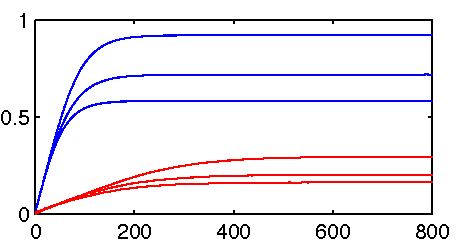
\includegraphics[scale=0.8]{history}\\
%& time~$t$
%\end{tabular}
%\caption{The histories of the mean velocity $\bq$ for the flow over the straight channel~(blue) and meandering channel~(red) at three reasonable observed stations. 
%The relevant parameters $2\beta=8$, $B=0.9$, $\kappa_1=1$, $\kappa_2=4\pi/L_x$, $\theta=0.01$~(straight) and $\theta=0.001$~(meander).
%Zero slopes of these curves indicate the fluid converges to steady state. }
%\label{history}
%\end{figure}%



This section focuses on the preliminary application of the model~\eqref{smag:h}--\eqref{smag:v} for turbulent flow driven by a small downslope along straight open channels.
The water covers the entire domain in order to avoid, at this stage, complications of moving contact lines between wet and dry bed: the flow is in the channel and over a surrounding flood plain.
We compare this turbulent channel flow with viscous open channel flow by Roberts et al.~\cite{Robertsli2006} and the experiments of turbulent flow over flood plains and channels in a flume with water of variable depth by Bousmar et al.~\cite{Bousmar2002,Bousmar2003a}.

Let~$x$ be the down-stream and $y$~be the cross-stream coordinate. 
%Consider the water of a depth~$h(x,y,t)$ flows with the averaged lateral velocities~$\uu(x,y,t)$ and~$\vv(x,y,t)$ along the channel of
We choose a quartic shape for the channel to make smooth transitions to and from the shallows and the channel: 
\begin{equation}
z=b(x,y)=-1+B-B\left\{\max\left[0,1-\left({y}/{\beta}\right)^2\right]\right\}^2,\label{bed:straight}
\end{equation}
where~$\beta$ denotes the half-width of the channel, $1-B$ the depth of water on the shallow `flood plain' on either side of the channel, and the mid-depth of the channel is one (non-dimensionally) as we set the mean water level to be at $z=0$.  
For the simulations reported here we set $2\beta=8$, $B=0.9$ so the shallows are of depth~$0.1$, and a mean slope $\theta=0.01$ in the $x$~direction.  
%Consider the initial still water level is zero and then the depth of the shallow regions is $-1+0.9=-0.1$.
For comparison, the channel of Bousmar~\cite{Bousmar2002} was about twice as deep in the constant channel as in the flood plain.

%Consider the fluid of zero initial water level flowing with small mean downstream velocity $\uu(x,y,t)$ down the open channel described by equation~\eqref{bed:straight}. 
%Nondimensionalise the variables of fluid depth $h(x,y,t)$ and mean lateral velocities $\uu(x,y,t)$ and $\vv(x,y,t)$ with respect to some velocity scale, a typical depth and a fluid density, and consider $g=1$. 
%Equations~\eqref{smag:h}--\eqref{smag:v} describe the dynamics of this fluid with the periodic boundary conditions both in the $x$~and~$y$ directions for both the flow and channel. 

Numerical simulations were simply implemented using centred difference approximations to the spatial derivatives in equations~\eqref{smag:h}--\eqref{smag:v} on a regular but staggered grid in space.
Time integration was performed by Matlab's \verb|ode15s|.

\begin{figure}
\centering
\begin{tabular}{cc}
\rotatebox{90}{\hspace{7ex}mean~$\uu$}&
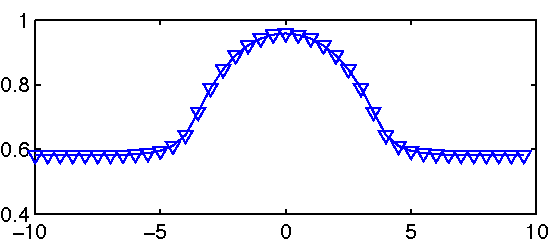
\includegraphics[scale=0.8]{straight-velocity-u}\\
& cross-section~$y$
\end{tabular}
\caption{Plot of the mean downstream velocity~$\uu$ in the cross-section at the point $x=20$ and the time $t=800$ with parameters $2\beta=8$, $B=0.9$ and $\theta=0.01$. 
The channel is nine times as deep as in the surrounding shallows, but the peak downstream velocity is only $50$\%~faster than in the shallows.}
\label{straight-velocity-u}
\end{figure}%

\begin{figure}
\centering
\begin{tabular}{c@{}c}
\rotatebox{90}{\hspace{9ex}\(y\)}&
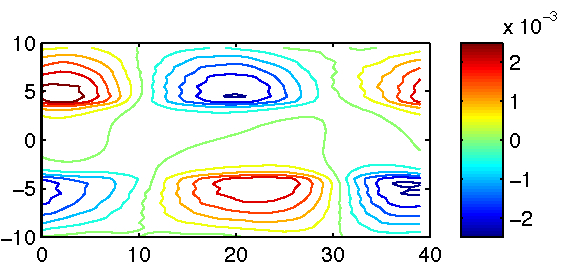
\includegraphics[scale=0.8]{straight-velocity-vc}\\
&\(x\)
\end{tabular}
\caption{Contours of the mean transverse velocity~$\vv$ at time $t=800$ with parameters $2\beta=8$, $B=0.9$ and $\theta=0.01$. 
The high value curves~(red) and low value curves~(blue) indicate travelling vortices on the shear near the interactions between the channel and shallow regions. }
\label{straight-velocity-vc}
\end{figure}%

\pdfcomment{Rule of thumb: generally put the figure environments immediately before the paragraph that the figure is first mentioned.}
In simulations, we typically started the fluid with zero velocity and a flat free surface ($z=0$). 
Transients in the simulations decayed on a non-dimensional time of typically $t=400$.
Figure~\ref{straight-velocity-u} shows that fast flow developed in the deeper channel and slow flow on the shallow regions.
In a viscous flow in a small open channel~\cite{Robertsli2006}, the flow was eight times as fast in the channel as on the shallow regions. 
Equation~\eqref{smag:u} suggests the equilibrium downstream velocity in the shallow regions is $\sqrt{0.993\sin(0.01)\times0.1/0.00293}=0.58$, which corresponds the numerical result in Figure~\ref{straight-velocity-u}. 
\pdfcomment{Avoid giving excessive decimal digits: prefer the minimum that is necessary.}
The equilibrium downstream velocity for a fluid of depth one is $\sqrt{0.993\sin(0.01)\times1/0.00293}=1.84$, but in our channel is only~$0.95$ as in Figure~\ref{straight-velocity-u}: 
such simulations show that when the shape of the bed becomes complex, the equilibrium downstream velocity decreases through lateral mixing and dissipation. 
For example, for the lesser slope~$\theta=0.001$, the equilibrium downstream velocity over a flat bed is~$0.58$, in mid-channel with  width~$2\beta=14$ is~$0.37$, in mid-channel with  width~$2\beta=8$ is~$0.30$, and in a slightly meandering channel with a width~$2\beta=8$ is~$0.31$.
Figure~\ref{straight-velocity-vc} displays the contour of the mean transverse velocity~$\vv(x,y,t)$ at time~$t=800$, which indicates that weak horizontal vortices grow on the shear in the transition between the channel and shallow regions.  
These weak mixing vortices travel downstream. 
Similar vortices were observed by Roberts and Li~\cite{Robertsli2006} in numerical simulations of viscous open channel flow and by Boussmar~\cite{Bousmar2003a} in experiments of turbulent flow along channels in a flume. 








\section{Flows along meandering channels}

This section describes simulations of turbulent flow over a slightly sloped ground with a meandering open channel. 
The simulations are compared with the numerical results of Liu et al.~\cite{Liu2009} and Demuren~\cite{Demuren1993} who calculated the two and three dimensional turbulence flows in meandering channels by a lattice Boltzmann model and a finite volume numerical model, respectively.

%Create a Cartesian coordinate system~$(x,y,z)$. 
%Consider nondimensionalised fluid depth $h(x,y,t)$, mean lateral velocities $\uu(x,y,t)$ in the $x$~direction and $\vv(x,y,t)$ in the $y$~direction. 
Here we describe simple meandering open channels by the bed
\begin{align}&
z=b(x,y)=-1+B-B\left\{\max\left[0,1-\left(\frac{y-\kappa_1\cos(\kappa_2x)}{\beta}\right)^2\right]\right\}^2,\label{bed:meander}
\end{align}
where the parameter~$\kappa_2$ determine the wavelength~$2\pi/\kappa_2$ of the meandering channel, the parameter~$\kappa_1$ is the half-width of the extent of the meanders, and the parameters $\beta$~and~$1-B$ are the half-width and mid-depth of the meandering channel as before.
Simulate the turbulent flow over such channel by the equations~\eqref{smag:h}--\eqref{smag:v} with periodic boundary conditions in both $x$~and~$y$ directions for both the flow and channel. 

\begin{figure}
\centering
\begin{tabular}{c@{}c}
\rotatebox{90}{\hspace{12ex}$y$}&
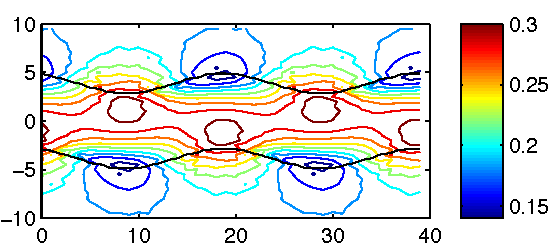
\includegraphics[scale=0.8]{meander-velocity-uc}\\
&$x$\\
\rotatebox{90}{\hspace{12ex}$y$}&
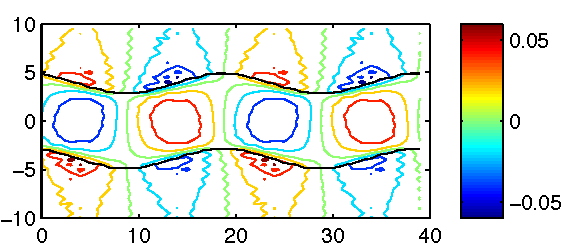
\includegraphics[scale=0.8]{meander-velocity-vc}\\
&$x$
\end{tabular}
\caption{Contours of the mean downstream velocity $\uu$~(top) and mean transverse velocity $\vv$~(bottom) at time $t=800$ with parameters $2\beta=8$, $B=0.9$, $\theta=0.01$, $\kappa_1=1$ and $\kappa_2=4\pi/L_x$. 
The black curves plot the meandering channel.}
\label{meander-velocity-cont}
\end{figure}%

%\begin{figure}
%\centering
%\begin{tabular}{c@{}c}
%\rotatebox{90}{\hspace{8ex}depth~$h$} &
%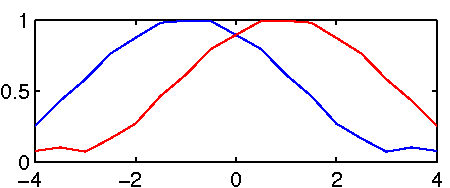
\includegraphics[scale=0.8]{meander-depth}\\
%& channel~cross-section~$y$
%\end{tabular}
%\caption{Plot of the fluid depth $h(x,y,t)$ in the cross-section of the channel at stations~$x=10$~(blue) and~$x=20$~(red). 
%The relevant parameters $2\beta=8$, $B=0.9$, $\theta=0.01$, $\kappa_1=1$ and $\kappa_2=4\pi/L_x$.}
%\label{meander-depth}
%\end{figure}%

In our numerical simulations, we found transients decay over times of typically \(t\approx400\).
Figure~\ref{meander-velocity-cont} exhibits the contours of the depth averaged lateral velocities $\uu(x,y,t)$~and~$\vv(x,y,t)$. 
The downstream velocity~$\uu$ reaches maximum at the bends.
The transverse velocity~$\vv$ attains maximum and minimum at the connection of the bends, which is consistent with the results of Liu eta al.~\cite{Liu2009} who modelled the water in meandering channels with~$60^\circ$ and~$90^\circ$ consecutive bends and a width of~$0.3$\,m.
Demuren~\cite{Demuren1993} calculated the water depth and the depth averaged longitudinal and transverse velocities of three dimensional flows in meandering channels with a natural bed configuration by a finite volume numerical method. 
Simulations at fifteen observed stations of the meandering channel indicate that the location of the maximum velocity shifts from the inner bank to the outer bank as the water flows through the bends of the channel. 

Plots of the water depth do not show any features of much interest: plots are dominated by the variations in the bed.
Figure~\ref{meander-velocity} plots of the the downstream velocity~$\uu(x,y,t)$ and the transverse velocity~$\vv(x,y,t)$ at the channel bends $x=10$ and $x=20$.
The downstream velocity and transverse velocity are bigger in the outer bank than in the inner bank, which correspond to the computations by Demuren~\cite{Demuren1993}. 


\begin{figure}
\centering
\begin{tabular}{c@{}c}
\rotatebox{90}{\hspace{6ex}mean~$\vv,\uu$} &
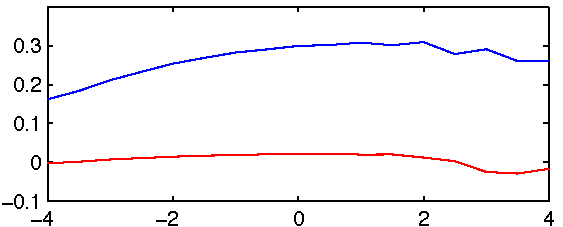
\includegraphics[scale=0.8]{meander-velocity1}\\
& channel~cross-section~$y$\\
\rotatebox{90}{\hspace{6ex}mean~$\vv,\uu$} &
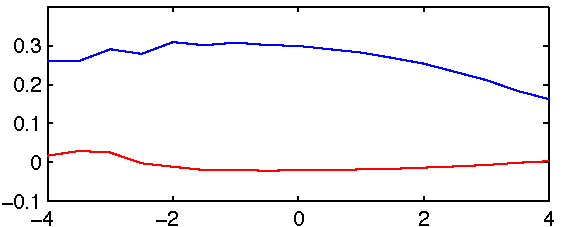
\includegraphics[scale=0.8]{meander-velocity2}\\
& channel~cross-section~$y$
\end{tabular}
\caption{The mean downstream velocity $\uu(x,y,t)$~(blue) and the mean transverse velocity $\vv(x,y,t)$~(red) in the cross-section of the channel at the bend $x=10$~(top) and $x=20$~(bottom). 
The relevant parameters $2\beta=8$, $B=0.9$, $\theta=0.01$, $\kappa_1=1$ and $\kappa_2=4\pi/L_x$.}
\label{meander-velocity}
\end{figure}%

\section{Conclusion}

The proposed approach to supporting turbulent flood models by the dynamical systems theory of centre manifolds appears to predict environmental turbulent fluids reliably. 
The flows in straight and meandering compound channel, as examples, were numerically simulated by the new approach. 
The results correspond to the analysis and numerical simulations of the published work~\cite[e.g.]{Bousmar2002, Liu2009}.
The equations~\eqref{smag:h}--\eqref{smag:v} account for the interactions between the vertical profiles and lateral spatial variations, and thus may in future work be used to better model erosion and sediment transport of the turbulent fluid.



\pdfcomment{Need to check and see if Bousmar's work has been published in a regular journal??}
\bibliographystyle{afmc}
\bibliography{bibsmag}
\end{document}